\section{Prompt-Based Approach}
\label{appraoch}
This section introduces our approach to generate the prompts needed for the code co-evolution. 
It first gives an overview of the approach. Then details the structure of the generated prompts, before to detail each part of it and how it is generated. Finally, it describes our prototype implementation.  

\begin{figure}
\centering
\hspace*{-0.8cm}
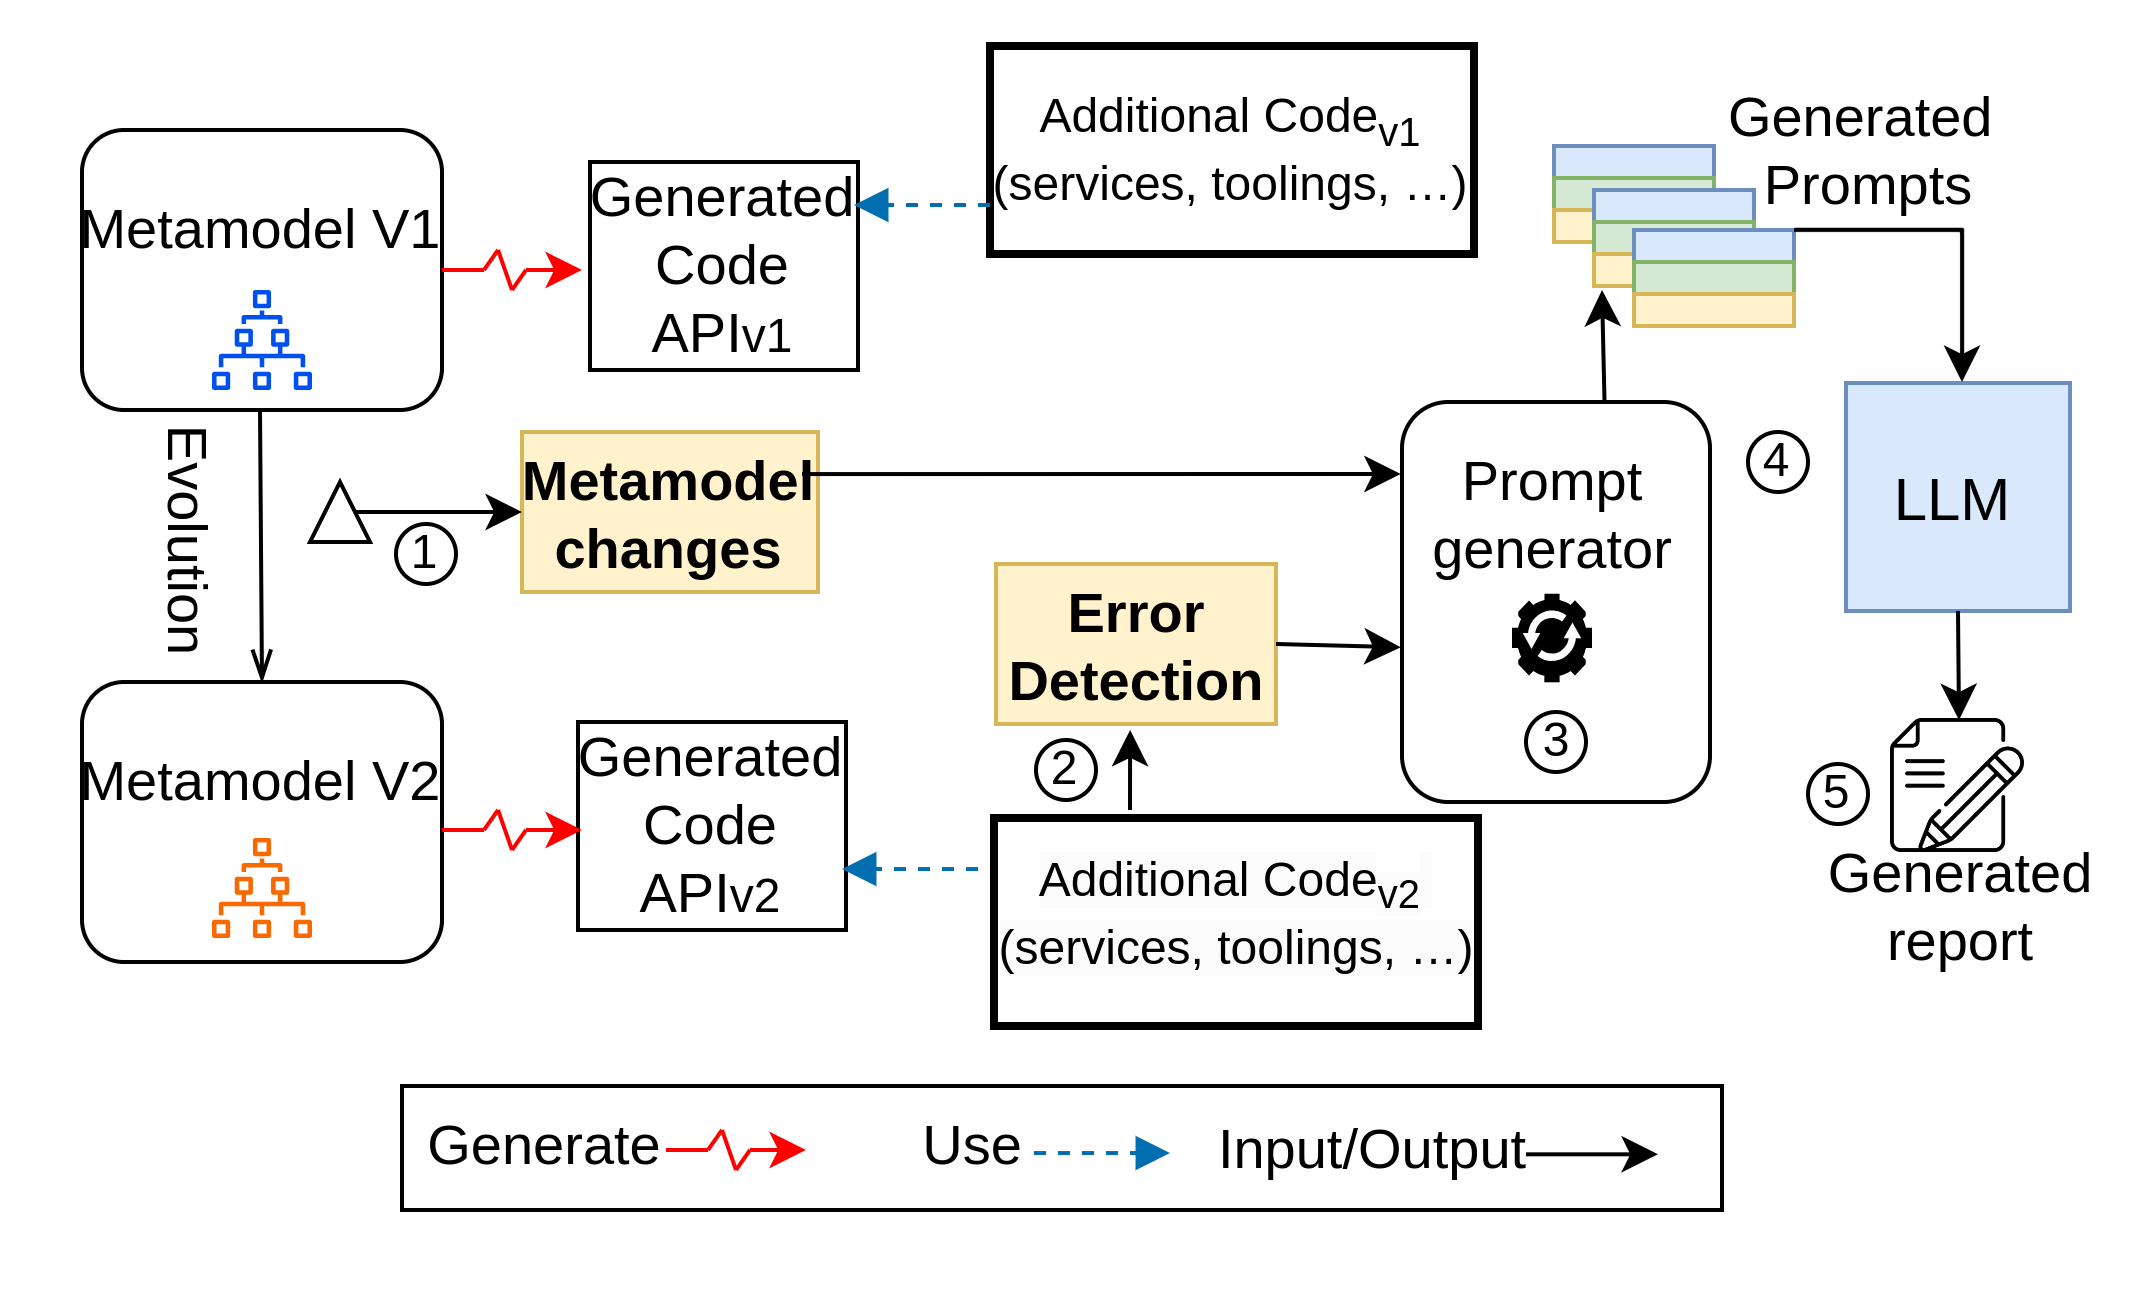
\includegraphics[width=0.55\textwidth]{pics/approach.png}
\caption{Overall Approach for Prompt-based co-evolution.}
\label{fig: approach}
%\vspace{-5mm}
\end{figure}



\subsection{Overview}

Figure \ref{fig: approach} shows the overall steps of our approach. We start by retrieving the list of changes that describe the evolution between the old metamodel and the new metamodel~\Circled{1}. 

When the metamodel evolves, the code API is regenerated, therefore the additional code is broken. The additional code is then parsed to collect the list of errors~\Circled{2}. The list of changes and the list of errors are the inputs of our prompt generator. The goal is to generate a prompt for each error, including sufficient information about the change and the error itself~\Circled{3}.
Each generated prompt is used to request ChatGPT to give a correction for the concerned error~\Circled{4}. A global report is generated for the additional code to allow the developer to have a visual output about the generated prompts and the answers of the LLM~\Circled{5}. Algorithm \ref{algo:overallalgo} further depicts the overall method of co-evolution based on a given LLM. After we parse the project, we retrieve the list of errors per class (Lines 2-3). Then for each error, we generate the prompt (Lines 4-5) and call the LLM and record its co-evolution response for analysis (Lines 6-7).
%\Circled{1}


\begin{algorithm2e}[t]
% \algsetup{linenosize=\tiny}
 \small
\SetAlgoLined
\KwData{EcoreModelingProject, changesList}
javaClasses $\leftarrow$ Parse(EcoreModelingProject)

\For {( jc $\in$ javaClasses)}
{
    errorsList $\leftarrow $ getErrors(jc)
    
    \For{(error : errorsList)}
    {
    prompt $\leftarrow$ promptGenerator(error, changesList, jc)
    
    coevolutionResponse $\leftarrow$ callLLM(prompt)
    
    addToReport(error, prompt, coevolutionResponse)
    }
}

 
 \caption{\LLM Co-evolution}
 \label{algo:overallalgo}
\end{algorithm2e}

\subsection{Generated Prompt Structure}

\begin{figure}[t]
\centering
%\hspace*{-1cm}
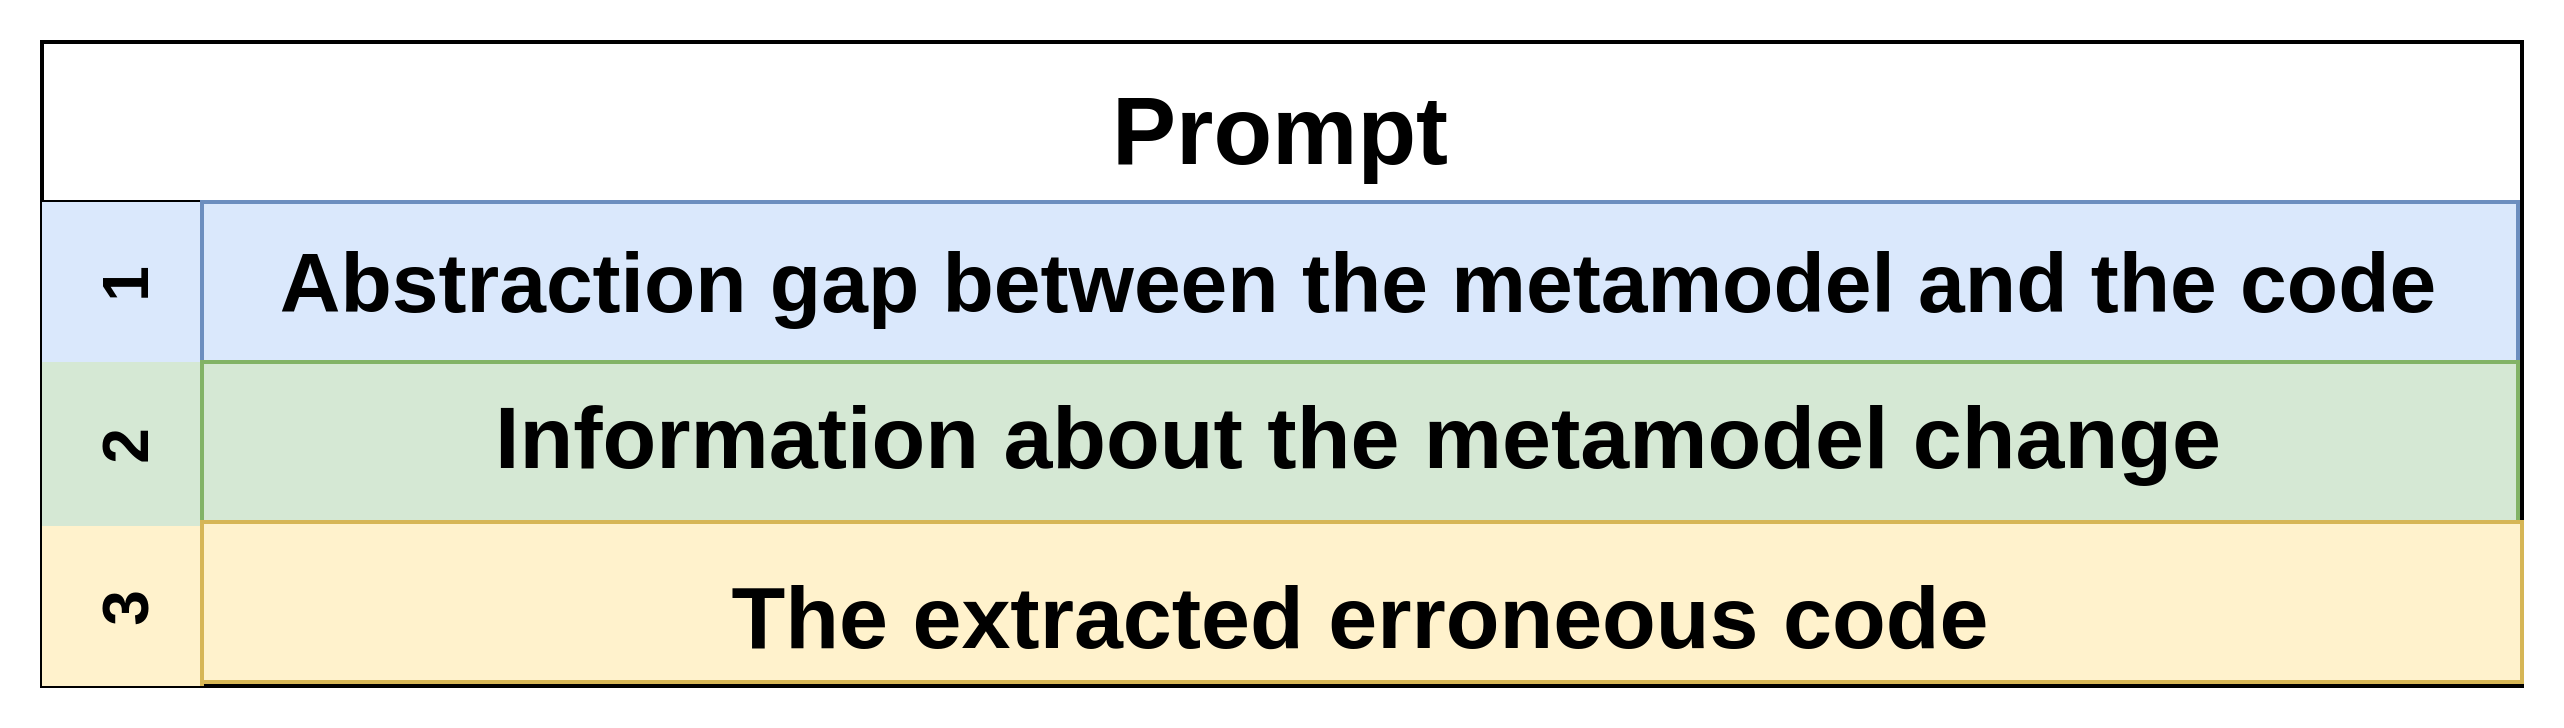
\includegraphics[width=0.5\textwidth]{pics/promptTemplate.png}
\caption{Generated Prompt Structure.}
\label{fig:promptstructure}
\vspace{-5mm}
\end{figure}

Figure \ref{fig:promptstructure} shows the overall structure of the envisioned prompts we will generate in order to co-evolve the code errors. In fact, the rationale behind the prompt structure is that our problem does not only concern the code errors to repair, but it is also related to the use of the code generated from the metamodels and their changes. Therefore, to contextualize our problem, we must explain :~1) what is the code generated from the metamodels,~2) what is the impacting metamodel change, and~3) what is the impacted code error to co-evolve.  Concerning the prompt prefix we use "Co-evolve this code" to ask \LLM for one co-evolution. Next subsections detail the different parts of the prompt structure. 

\subsection{Abstraction Gap Between Metamodels and Code}

One main distinction from simply repairing code errors is the interplay between the metamodels and the additional code through the generated code from the metamodels. This is due to the gap in abstraction in between metamodels and generated code. In fact, for each metamodel various code elements are generated for each metamodel element and with different patterns.
Table~\ref{table:locationofMMelemen} classifies and provides illustrative examples for the different generated code elements from each metamodel element, namely metaclass, attribute/reference, and method.  %It shows that various code elements are generated for each metamodel element type and with different patterns. 
%%mapping between the different metamodel elements and their corresponding generated code elements with illustrative examples. 
For example, take the case of a metaclass\footnote{For simplicity, we refer to a metaclass by simply a class in the remaining of the paper.}. EMF generates a corresponding interface and a class implementation, a \emph{createClass()} method in the factory class, three literals (\ie constants) for the class and an accessor method in the package class, and a corresponding to create adapter method. For the attribute case, EMF generates the signature and implementation of a getter and a setter, an accessor, and a literal. 
%This classification is essential to match the different errors with their corresponding pattern usages in the code, before to co-evolve them with the appropriate resolution strategy. 
This classification is essential to match the different errors with the right used generated code elements to explicit the abstraction gap. \red{If a class is changed, all its generated elements are impacted and their usages will be erroneous. For example, if a class is renamed, every invocation of the method "get+className" will be erroneous and must be co-evolved}. Thus, we consider the abstraction gap as the first contextual information we inject in the prompts for the LLM to co-evolve the code errors. 


\begin{table*}[t]

\caption{Classification of the different patterns of the generated code element from the metamodel elements. \\\hspace{3em} [Examples illustrated for a metaclass \emph{Rule}, property \emph{Status}, and method \emph{Execute()}]} 

\label{table:locationofMMelemen}
	\resizebox{17cm}{!} {
{\small
\begin{tabular}{llll}
\toprule

\begin{tabular}[c]{@{}l@{}} \textbf{Metamodel}\\ \textbf{element type} 
\end{tabular} & \textbf{Generated code elements}& \textbf{Pattern of the generated code elements}& \textbf{Examples}\\ \midrule


\multirow{6}{*}{Metaclass} & Interface & "MetaClassName" & \textit{Rule} \\ \cline{2-4} 
 & \begin{tabular}[c]{@{}l@{}}createClass() \\ (in metamodelFactory class)\end{tabular} & "create"+"MetaClassName"() &\textit{createRule()} \\ \cmidrule{2-4} 
 & \begin{tabular}[c]{@{}l@{}}Literals of the class \end{tabular} &
 \begin{tabular}[c]{@{}l@{}}
 "META\_CLASS\_NAME"\\
 "META\_CLASS\_NAME"+"\_"+ "FEATURE\_COUNT"\\
 "META\_CLASS\_NAME"+ "\_"+"OPERATION\_COUNT"
 \end{tabular} 
 & \begin{tabular}[c]{@{}l@{}}\textit{RULE}, \\ \textit{RULE\_FEATURE\_COUNT}, \\  \textit{RULE\_OPERATION\_COUNT}\end{tabular} \\ \cmidrule{2-4} 
 & \begin{tabular}[c]{@{}l@{}}Accessor of Meta objects \\ (in metamodelPackage class)\end{tabular} & "get"+"MetaClassName"()& \textit{getRule() }\\ \cmidrule{2-4} 
 & Class implementation & "MetaClassNameImpl" &\textit{RuleImpl }\\ \cmidrule{2-4} 
 & Adapter & "create"+"MetaClassName"+"Adapter" & \textit{createRuleAdapter()} \\ \midrule


\multirow{1}{*}{Attribute} & Signature of getters and setters & "get"+"AttributeName"(), "set"+"AttributeName"()& \textit{getStatus()}, \textit{setStatus() }\\ \cmidrule{2-4} 
\multirow{2}{*}{(Same for a} & Accessor of Meta objects &"get"+"MetaClassName"+"\_"+"AttributeName"() &\textit{getRule\_Status()} \\ \cmidrule{2-4} 
\multirow{1}{*}{Reference)}  & Literal & "META\_CLASS\_NAME"+"\_\_"+"ATTRIBUTE\_NAME"& \textit{RULE\_\_STATUS} \\ \cmidrule{2-4} 
 & \begin{tabular}[c]{@{}l@{}}Implementation \\ of getters and setters\end{tabular} &"get"+"AttributeName"(), "set"+"AttributeName"()& getStatus(), setStatus() \\ \midrule


\multirow{4}{*}{Method} & Declaration of the method& "methodName"()& \textit{Execute() }\\ \cmidrule{2-4} 
 & Accessor of meta objects &"get"+"MetaClass"+"\_\_"+"MethodName"()& \textit{getRule\_\_Execute() }\\ \cmidrule{2-4} 
 & Literal &"META\_CLASS\_NAME"+"\_\_"+"METHOD\_NAME"& \textit{RULE\_\_\_EXECUTE}\\ \cmidrule{2-4} 
 & Implementation of the method &"methodName"()& \textit{Execute()} \\ %\midrule


%\multirow{4}{*}{Reference} & Accessor of meta objects &"get"+"MetaClassName"+"\_"+"ReferenceName"()& \textit{getConstraint\_ConstraintElement()} \\ \cmidrule{2-4} 
% & Signature of getters and setter & "get"+"ReferenceName"(),"set"+"ReferenceName"()&\textit{ getConstraintElement()}, \textit{setConstraintElement() }\\ \cmidrule{2-4} 
% & Literal &"META\_CLASS\_NAME"+"\_\_"+"REFERENCE\_NAME"& \textit{CONSTRAINT\_\_CONSTRAINT\_ELEMENT} \\ \cmidrule{2-4} 
% & \begin{tabular}[c]{@{}l@{}}Implementation of \\ getters and setters\end{tabular} &"get"+"ReferenceName"(), "set"+"RegerenceName"()& \textit{getConstraintElement()}, \textit{setConstrainElement() }\\ 
\bottomrule
 
 %cline hline replaced with cmidrule and midrule
 
\end{tabular}
}
}
\end{table*}



\subsection{Metamodel Evolution Changes}
 \label{mmchanges}
A metamodel represents a high abstraction level of a domain.
Like any software artefact, metamodels evolve to meet domain changing requirements \cite{mens2008introduction}.
Herrmannsdoerfer et al. \cite{Herrmannsdoerfer2011} distinguish two types of metamodel changes: \emph{atomic} and \emph{complex}. Atomic changes are additions, removals, and updates of a metamodel element. Complex changes consist of a combination of atomic changes ~\cite{vermolen2011reconstructing,khelladi2015detecting}. 
%
For example, push property is a complex change where a property is pushed from a parent class to an inheriting child class. This is composed of two atomic changes: delete a property and add a property~\cite{Herrmannsdoerfer2011}. 
Many approaches in the literature~\cite{Alter2015, williams2012searching,cicchetti2009managing,langer2013posteriori,vermolen2011reconstructing,Khelladi2016,bettini2022executable} exist to detect metamodel changes between two versions. 
\red{Particularly in our work, we use \cite{Khelladi2016,khelladi2016ad} to extract the changes between two metamodel versions. }

In practice, we focus on the impacting metamodel changes that will require co-evolution of the code and not on the non-impacting changes. For example, an add change of a class does not require co-evolution. However, a delete change or a change of type will impact the code that must be co-evolved. 
%Table \ref{xyz} gives 
The list of impacting metamodel changes \cite{iovino2012impact,cicchetti2009managing} we consider in the prompts is as follows: \emph{1)} Delete property\footnote{Property refers to Attribute, Reference, and Method.} \emph{p} in a class \texttt{C}, \emph{2)} Delete class \texttt{C}, \emph{3)} Rename element \emph{e} in a class \texttt{C}, \emph{4)} Generalize property \emph{p} multiplicity from a single value to multiple values in a class \texttt{C},  \emph{5)} Move property \emph{p} from class \texttt{Source} to \texttt{Target} through a reference \emph{ref},  \emph{6)} Extract class of properties $p_{1},...,p_{n}$ from \texttt{Source} to \texttt{Target} through a reference \emph{ref},  \emph{7)} Push property \emph{p} from super class \texttt{Super} to sub classes \texttt{Sub$_{1}$},...,\texttt{Sub$_{n}$}, \emph{8)} Inline class \texttt{Source} to \texttt{Target} with properties $p_{1},...,p_{n}$, and \emph{9)} Change property \emph{p} type from \texttt{S} to \texttt{T} in a class \texttt{C}. 

\begin{comment}
    \item \emph{1)} Delete property\footnote{Property refers to Attribute, Reference, and Method.} \emph{p} in a class \texttt{C}. 
    
    \item \emph{2)} Delete class \texttt{C}. 
    
    \item \emph{3)} Rename element \emph{e} in a class \texttt{C}. 
    
    \item \emph{4)} Generalize property \emph{p} multiplicity from a single value to multiple values in a class \texttt{C}. 
    
    \item \emph{5)} Move property \emph{p} from class \texttt{Source} to \texttt{Target} through a reference \emph{ref}. 
    
    \item \emph{6)} Extract class of properties $p_{1},...,p_{n}$ from \texttt{Source} to \texttt{Target} through a reference \emph{ref}. 
    
    \item \emph{7)} Push property \emph{p} from super class \texttt{Super} to sub classes \texttt{Sub$_{1}$},...,\texttt{Sub$_{n}$}. 
    
    \item \emph{8)} Inline class \texttt{Source} to \texttt{Target} with properties $p_{1},...,p_{n}$. 
    
    \item \emph{9)} Change property \emph{p} type from \texttt{S} to \texttt{T} in a class \texttt{C}. 
\end{comment}

Thus, we consider these definitions of metamodel changes as the second contextual information we inject in the prompts for the LLM to co-evolve the code errors. 

%\emph{1)} Delete property \emph{p} in a class \texttt{C}. \emph{2)} Delete class \texttt{C}.\emph{3)} Rename element \emph{e} in a class \texttt{C}. \emph{4)} Generalize property \emph{p} multiplicity from a single value to multiple values in a class \texttt{C}. \emph{5)} Move property \emph{p} from class \texttt{S} to \texttt{T} through a reference \emph{ref}. \emph{6)} Extract class of properties $p_{1},...,p_{n}$ from \texttt{S} to \texttt{T} through a reference \emph{ref}. \emph{7)} Push property \emph{p} from super class \texttt{Sup} to sub classes \texttt{Sub$_{1}$},...,\texttt{Sub$_{n}$}. \emph{8)} Inline class \texttt{S} to \texttt{T} with properties $p_{1},...,p_{n}$. \emph{9)} Change property \emph{p} type from \texttt{S} to \texttt{T} in a class \texttt{C}.


\subsection{Extracted Code Errors}

Now that we have two main ingredients needed for the generation of the prompts. %, namely metamodel changes and the abstraction gap between metamodels and code. 
We only require the erroneous code to be co-evolved. 

To do so, we parse the code (i.e., \emph{compilation units}) to access the Abstract Syntax Trees (ASTs) and retrieve the code errors. %An error in a Java code is called a \emph{Marker} that contains the information regarding the detected error. It
Each error contains the necessary information to locate the exact impacted AST node in the parsed global AST (\ie char start and end) and to process it (\ie message). 
After that, we simply extract the sub-AST corresponding to the code containing the error. 
We consider three possible situations, namely 1) if the error is in a method, we extract the whole method, 2) if the error is in the imports, we extract the list of imports, 3) if the error is in the class definition or the fields, we extract it without the class's methods. This constitutes the final part of the contextual information we inject in the prompts for the LLM to co-evolve the code errors. Note that we simply specify in the prompt before the code the order to \emph{"Co-evolve this code: "}.
%\red{This prefix is selected after trying other terms like "update" and "correct" because it is more related to our problem.}.

%In the remaining part of the paper, we refer to errors and Java classes for the sake of simplicity. 


%\begin{figure}[t]\centering%
%\scalebox{0.9}{\small\input{pics/PromptStructure}}
% \vspace*{-0.3cm}
%\caption{Generated Prompt Structure.}
%\label{fig:promptStruct}
%\vspace{-1em}
%\end{figure}

\subsection{Prompt Generation}
\label{promptgeneration}

Algorithm~\ref{algo:promptgenerator} allows generating prompts following the specified structure in Figure~\ref{fig:promptstructure}. It first finds the ASTNode corresponding to the error in the code (Line~1). Then, it iterates over the list of metamodel changes to match  the error node with the code usage to identify the impacted abstraction gap (Lines~6-8). After that, it summarizes the impacting metamodel change (Line~11). Finally, it extracts the erroneous code (Line~21) and puts together all three contextual information into one generated prompt (Lines~22-25). 
%
Figure~\ref{fig:promptexample} shows an example of the generated prompt for the error in Listing~\ref{lis:Modisco_Code_External_V1} (Line~4) due to the move of property \emph{DiscoveryTimeInSeconds} in the metamodel.  

\begin{figure}[t]
\centering
%\hspace*{-1cm}
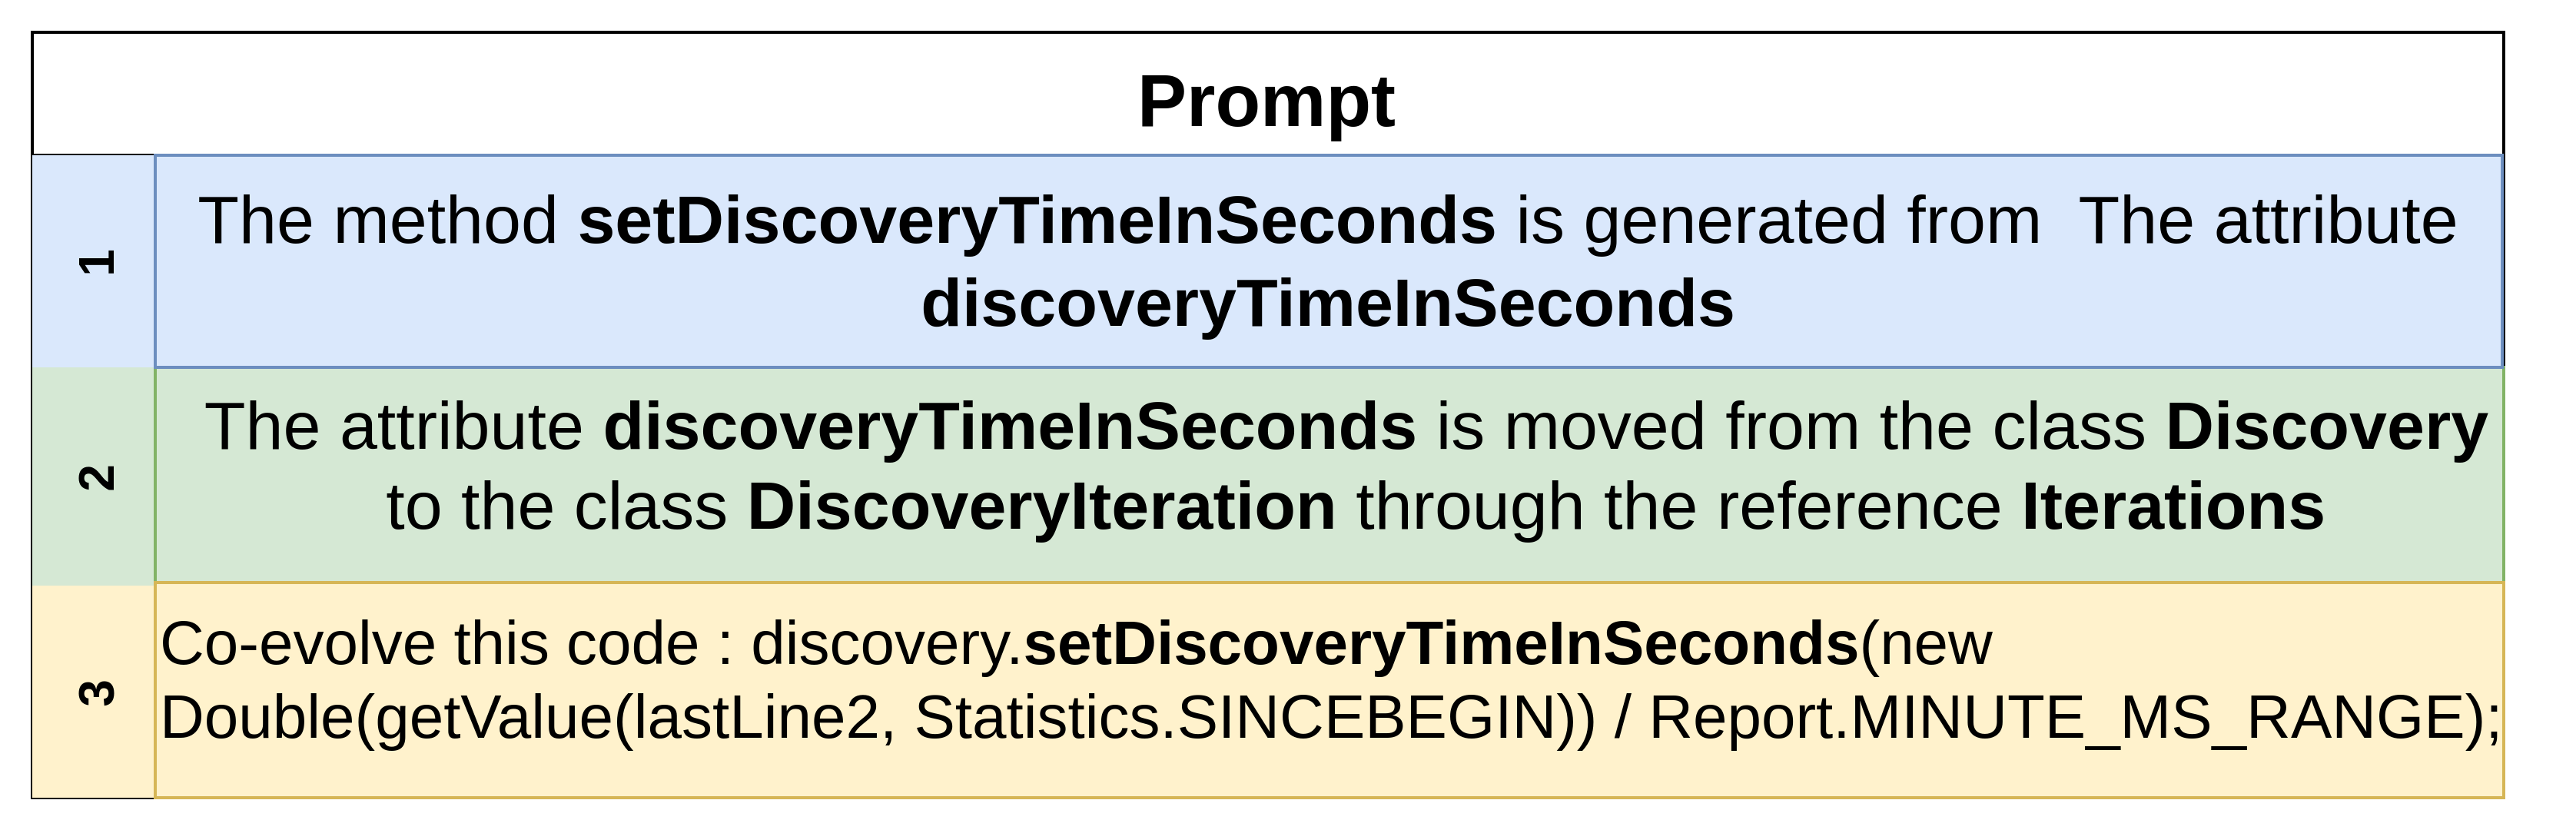
\includegraphics[width=0.5\textwidth]{pics/PromptStructure.png}
\caption{Move attribute prompt example.}
\label{fig:promptexample}
\vspace{-5mm}
\end{figure}

 
\begin{algorithm2e}[t]
% \algsetup{linenosize=\tiny}
 \small
\SetAlgoLined
\KwData{error, changesList, javaClass}
    
    errorNode $\leftarrow$ findErrorAstNode(javaClass, error)
       
    found $\leftarrow$ false
    
    %\uIf{(errornode.isTypeOf( SimpleName))}
    		%{
    		\While {(change  $\in$ changesList $\&$ $\neg found$)}
            {
    		\Switch{change}{
                \Case{RenameClass}{%V errornode.name="set"+change.name)
                    \uIf{(errornode.name="get"+change.name )}
                    {
    found $\leftarrow$ true  
    
    abstractionGap="The method "+ errornode.name+" is generated from the metaclass "+ change.name
                     } 
                     \uElseIf {...}{\emph{\textcolor{circlegreen}{/*treat other abstraction gaps*/}}}
    changeInfo= "The metaclass "+ change.oldName+" is renamed to "+change.newName
                }
                \Case{RenameProperty}{
                    ...
                }
                \Case{DeleteProperty}{
                    ...
                }
                }
    
    
    		}
		%} \uElseIf {( errornode.isTypeOf( QualifiedName))}
		%{	  \emph{\textcolor{circlegreen}{/*repeat same matching process*/}}
		%...
        %}


codeError $\leftarrow$ extractCodeError(errornode)

prompt.add(abstractionGap)

prompt.add(changeInfo)

prompt.add(codeError) 
    
\textbf{return} prompt

\caption{Prompt Generator Algorithm}
\label{algo:promptgenerator}
\end{algorithm2e}


\begin{comment}

 
\begin{algorithm2e}[t]
% \algsetup{linenosize=\tiny}
 \small
\SetAlgoLined
\KwData{error, changesList, javaClass}

    errorNode $\leftarrow$ findErrorAstNode(javaClass, error)
       
    \uIf{(errornode.isTypeOf( SimpleName))}
    		{
    		\For {(change  $\in$ changesList)}
            {
    		\Switch{change}{
                \Case{RenameClass}{%V errornode.name="set"+change.name)
                    \uIf{(errornode.name="get"+change.name )}
                    {
   request="The method "+ errornode.name+" is generated from the metaclass "+ change.name
                           +" That is renamed from " +change.name+ " to "+change.newName
                     }   
                }
                \Case{RenameProperty}{
                    ...
                }
                \Case{DeleteProperty}{
                    ...
                }
                }
    		}
		} \uElseIf {( errornode.isTypeOf( QualifiedName))}
		{	  \emph{\textcolor{circlegreen}{/*repeat same matching process*/}}
		...
        }
    code$\leftarrow$getCode(errornode)

    prompt.add(request)
    
    prompt.add(code)
    
\textbf{return} prompt
 \caption{Prompt generator algo}
 \label{algo:promptgenerator}
\end{algorithm2e}

 
\end{comment}



%\subsection{Prototype Implementation}

\subsection{Prototype Implementation}
We implemented our solution as an eclipse Java plugin handling Ecore/EMF metamodels and their Java code. To retrieve the list of errors, we used JDT eclipse plugin \footnote{Eclipse Java development tools (JDT): \url{https://www.eclipse.org/jdt/core/}}. To launch our tool, we added a command to the context menu when selecting a java project. Generated prompts are sent to \LLM (see next section \ref{selectedLLM}), more specifically, its OpenAI API endpoint "https://api.openai.com/v1/chat/completions". We used Java JSON package to send our prompts and to receive \LLM responses. The error location, the corresponding generated prompt and \LLM responses are parsed in CSV file to have a visible results and to keep the history of proposed the co-evolutions.
Moreover, quick fixes (our baseline) are called using 
\textit{org.eclipse.jdt.ui.text.java.IQuickAssistProcessor} and \textit{org.eclipse.jdt.ui.text.java.IJavaCompletionProposal}.